\section{Data Gathering}
The following stronglines were targeted for each element: \\
\\
Barium: 4554 \AA \\
Europium: 3819, 3907, 4129, 4205 \AA \\
Lanthanum: 3949 \AA \\
\\
Due to data ranges and overall readability of some spectral lines, the number of stronglines varied for each of the three elements. For elements with multiple stronglines within the data range, we computed an average abundance across the computed abundances.

The abundances were computed using the astrophysics software MOOG \cite{moog}, which performed a stellar line analysis on the initial dataset.

Once the data was gathered and computed for the initial dataset, we then utilized literature searches for Barium, Europium, and Lanthanum in similar red giant field stars. This literature data was then used to supplement our existed computations, and help further define the trends within the data. As the majority of the literature data presented element abundances in $\frac{X}{Fe}$ units, with X being the respective element, we decided to use these units for our entire dataset. As our initial dataset, computed with MOOG, was in the $log\epsilon$ unit, we performed a conversion from $log\epsilon$ to $\frac{X}{Fe}$, shown in Figure \ref{eq:conversion}.

\section{Results}

For each element, the abundances were graphed against the respective metallicity of the red giant field star, shown in Figures \ref{Ba_v_Metal} - \ref{La_v_Metal}.

\begin{figure}[H]
  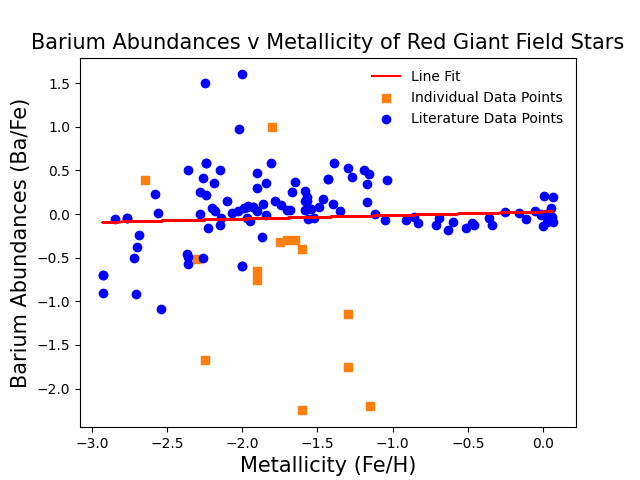
\includegraphics[width=\textwidth]{Ba_v_Metal.png}
  \caption{A graph of Barium abundances v. Metallicity of red giant field stars}
  \label{Ba_v_Metal}
\end{figure}

\begin{figure}[H]
  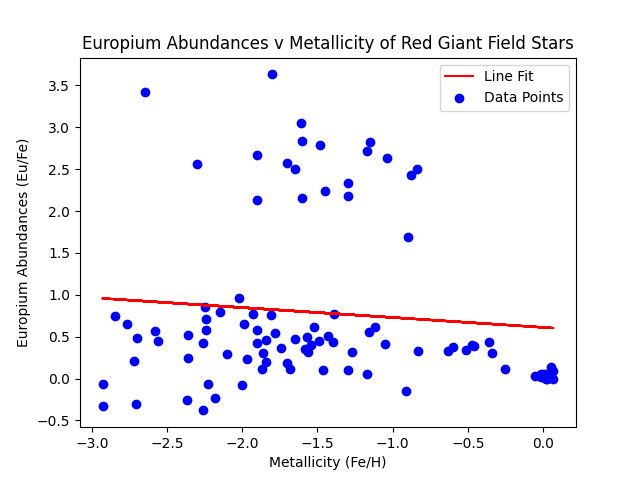
\includegraphics[width=\textwidth]{Eu_v_Metal.png}
  \caption{A graph of Europium abundances v. Metallicity of red giant field stars}
  \label{Eu_v_Metal}
\end{figure}

\begin{figure}[H]
  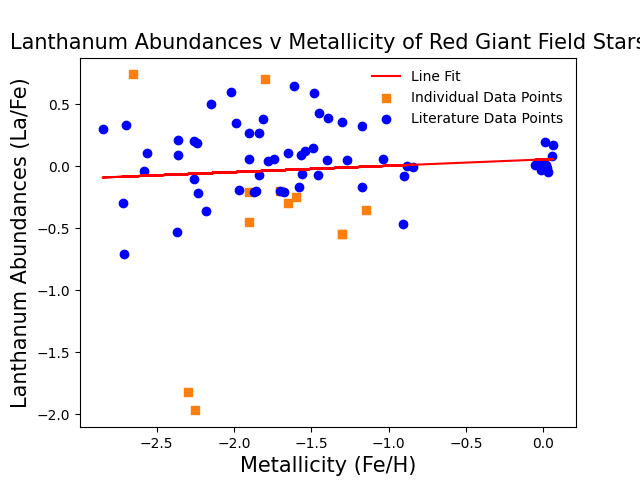
\includegraphics[width=\textwidth]{La_v_Metal.png}
  \caption{A graph of Lanthanum abundances v. Metallicity of red giant field stars}
  \label{La_v_Metal}
\end{figure}

The resulting graphs of element abundances v star metallicity can be further analyzed to interpret the effects of the r- and s-process. As the metallicity of a star is in relation to our Sun's metallicity, a more 'negative' value representsa smaller metallicity than the Sun, whereas a more 'positive' value represents a larger metallicity. In our own galaxy, the age of stars is related to the overall metallicity, with older stars having a more negative metallicity, and younger stars having a more positive metallicity.

Europium, shown in Figure \ref{Eu_v_Metal}, clearly shows Europium's dependance on the r-process. In the younger stars, with metallicity ~0.0, there is less overall mixing in the galaxy and therefore showing a more concentrated abundance of Europium. As we look towards the older stars ~3.0 metalicity, we can see a slight smoothing of overall abundances due to mixing, but there is no real boost in element abundance. This proves that Europium abundances are mainly due to the r-process.

Lanthanum, shown in Figure \ref{La_v_Metal}, tells a similar story. In the younger stars, there is less mixing, giving a more concentrated abundance due to the r-process. In the older stars, the abundances have mixed, but the overall abundance is similar to the values in the younger stars. There is a slight boost, however, due to the s-process, which 'kicks' in the older stages of the stars' lives. 

Barium, shown in Figure \ref{Ba_v_Metal}, differs from Lanthanum and Barium in that it is dominated by the s-process in the later stages of the stars' lives. The early stages are similar to Lanthanum and Barium, but there is a large jump in abundances once the s-process has had time to 'kick' in, after billions of years.

The relationships of the three heavy elements can also be expressed through comparisons, shown in Figures \ref{Ba_v_Eu} - \ref{Eu_v_La}.

\begin{figure}[H]
  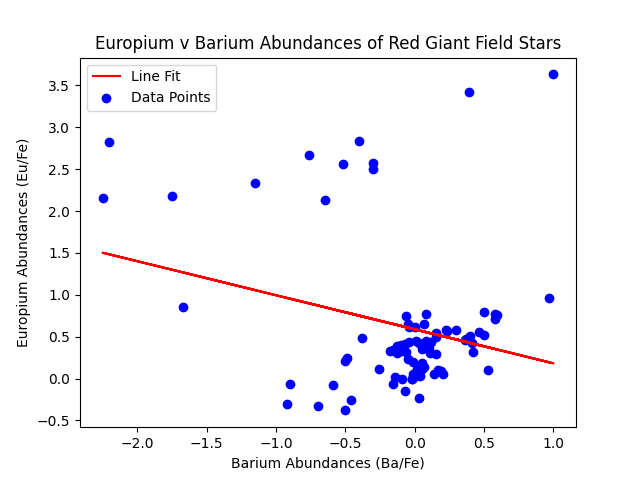
\includegraphics[width=\textwidth]{Ba_v_Eu.png}
  \caption{A graph of Barium v. Europium abundances of red giant field stars}
  \label{Ba_v_Eu}
\end{figure}

\begin{figure}[H]
  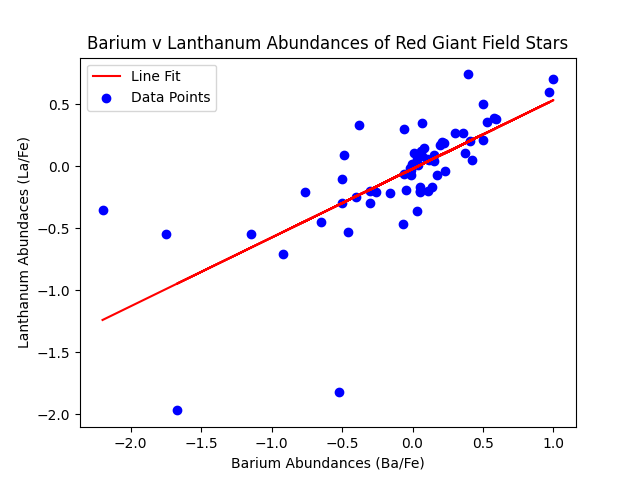
\includegraphics[width=\textwidth]{Ba_v_La.png}
  \caption{A graph of Barium v. Lanthanum abundances of red giant field stars}
  \label{Ba_v_La}
\end{figure}

\begin{figure}[H]
  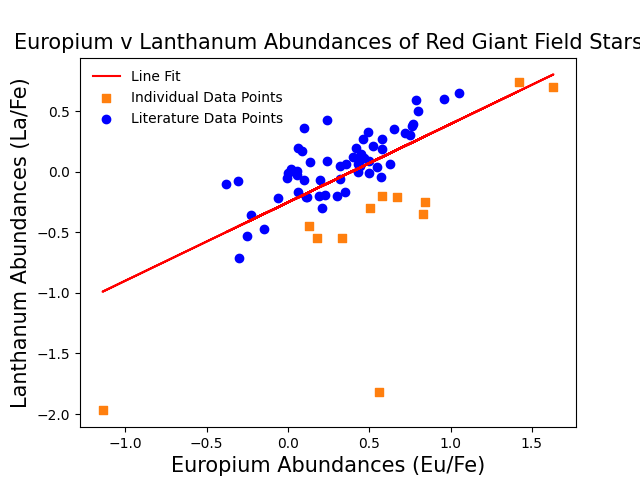
\includegraphics[width=\textwidth]{Eu_v_La.png}
  \caption{A graph of Europium v. Lanthanum abundances of red giant field stars}
  \label{Eu_v_La}
\end{figure}

The relationship between Lanthanum and Barium, shown in Figure \ref{Ba_v_La}, is especially telling of the contributions from the r- and s-process. The relationship between the two elements' abundances is nearly linear, showing how both elements gain at first from the r-process, and then later from the s-process.

Europium and Barium, shown in Figure \ref{Ba_v_Eu}, is not nearly as linear, instead showing the relatively low abundance of Europium when compared to Barium. This shows the reliances of Europium on the r-process, whereas Barium gains from both the r- and s-process, causing a growing abundance over time while Europium stays stagnant. Europium and Lanthanum tells a similar story, with Lanthanum growing over time due to the r-process, whereas Europium stays similar to its starting abundances.

\section{Conversions}

The conversion from $log\epsilon$, used by the original MOOG dataset, to $\frac{X}{Fe}$, used by the majority of literature datasets, is shown in Figure \ref{eq:conversion}.

\begin{figure}[H]
  \[\frac{X}{Fe} = log\epsilon(X) - 12 - \frac{Fe}{H} - \frac{X}{Fe}_{solar} \]
  \caption{Equation for $log\epsilon$ to $\frac{X}{Fe}$ conversion, with X being the current element, $\frac{Fe}{H}$ being the metallicity of the respective star, and $\frac{X}{Fe}_{solar}$ being the current element solar abundance}
  \label{eq:conversion}
\end{figure}

